\documentclass[11pt,oneside]{amsart}
\usepackage{geometry}                % See geometry.pdf to learn the layout options. There are lots.
\geometry{letterpaper}                   % ... or a4paper or a5paper or ... 
%\geometry{landscape}                % Activate for for rotated page geometry
%\usepackage[parfill]{parskip}    % Activate to begin paragraphs with an empty line rather than an indent
\usepackage{graphicx}
\usepackage{amssymb}
\usepackage{epstopdf}
\usepackage{hyperref}
\usepackage{pdfpages}
\DeclareGraphicsRule{.tif}{png}{.png}{`convert #1 `dirname #1`/`basename #1 .tif`.png}

\title{The Bar Buddy}
\author{Cliff Braun}
\date{December, 13, 2016}                                           % Activate to display a given date or no date
\begin{document}
\maketitle

\begin{figure}[htbp]
\begin{center}
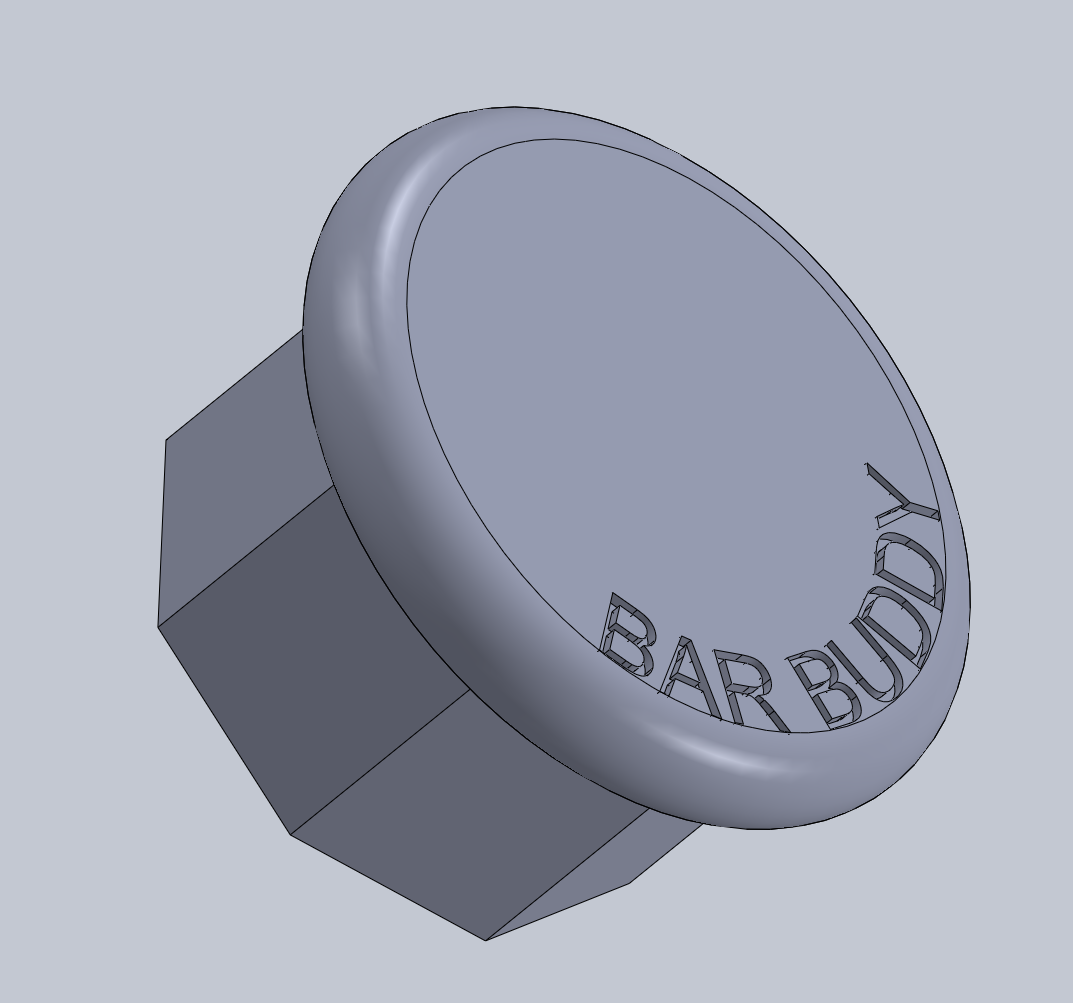
\includegraphics[width=\textwidth]{figures/barbuddy.png}
\end{center}
\end{figure}

\newpage
\tableofcontents
\section{Introduction}
The Bar Buddy provides a motion analytics system to the weightlifter. There are two potential groups of customers for the product, that entail very different software implementation and interface, but very similar hardware requirements. The two groups are those seeking to automatically track their workouts, and more serious athletes looking for motion analytics to improve their form. Some hardware exists already to fulfill this function, but requires a physical tether from barbell to floor unit (\url{http://www.roguefitness.com/open-barbell-v2}).
\subsubsection{Automated Workout Tracking}
The largest group of potential customers is normal gym goers, who are looking for an easier way to track their workouts. Counting to ten becomes a challenge when working very hard. Beyond basic tracking functionality this market could be expanded by a prescribed workout app. The customer could perform listed exercises and watch as they are counted on screen, potentially with helpful feedback.
\subsubsection{Advanced Motion Analytics}
A smaller, but perhaps more interesting from an engineering standpoint, application is that of advanced motion analytics. This application would allow an athlete to receive real-time input on form. Potential examples of this include comparing workouts week over week for speed and stability, correcting poor form, and even suggesting auxiliary exercises to strengthen detected deficiencies.
\section{Specifications}
System specifications are shown in Table \ref{tab:spec}
\begin{table}[htp]
\caption{System Requirements}
\begin{center}
\begin{tabular}{|c|c|}
\hline
System& Requirement\\
\hline
Maximum Acceleration & 10g\\
\hline
Minimum activity spacing & 0.1s\\
\hline
Battery life & 8h\\
\hline
Environmental Monitoring & Temp \& Humidity\\
\hline
User interface & Wireless (Ideally BTLE)\\
\hline
\end{tabular}
\end{center}
\label{tab:spec}
\end{table}%

\section{Design Development}
\subsection{WiPy Hardware Design}
Initial hardware design was performed with the intent to use the "WiPy" microcontroller. This micro was chosen because of its support for MicroPython, built in WiFi, and meeting all other design requirements.  The schematic created for this board is shown in Section \ref{sec:schematic}. The board consists of three major subsystems: power management, sensor support, and debug.
\subsubsection{Power Management}
Power for the system is provided from a standard 3.7V lithium polymer battery or the USB bus. The board contains a LT-1129 voltage regulator to convert battery voltages to the system voltage of 3.3V. A self-contained MCP73831T lithium polymer is also on board. Both the battery voltage and charger state are routed through voltage dividers to analogue input pins to allow system monitoring.
\subsubsection{Sensors}
The primary purpose of the board is to interface I2C motion and environment sensors to the micro controller to allow for data collection. The sensors utilized are the Bosch BNO055 integrated motion unit, and a Silicon Labs 7021 temperature and relative humidity sensor. These sensors share an I2C bus and associated hardware. The board provides mounting for an external crystal and associated components to increase accuracy of the BNO. An odd quirk of routing constraints: the BNO's I2C\_ADDR\_SEL signal is routed through a WiPy pin to allow for knitting of ground planes.
\subsubsection{Debug}
A CP2102 USB to UART bridge was included in an effort to ease system debugging as a micro-USB power was already included in the board for charging purposes. This component is relatively simple in use, but slightly complicates routing. USB signals should be routed on differential pairs, and incorporating ESD suppression diodes in the routing posed a challenge.
\subsection{BeagleBone Hardware ``Design''}
During hardware bring-up the WiPy host board was put into an unworkable state, necessitating a redesign to allow for collection of data. The redesign was of greatly reduced scope, mainly aiming to validate that the Bosch sensor was capable of providing useful data for the product concept. The Beaglebone Black was chosen as the host for practical reasons: one was in the bin-o'-micros, and the Raspberry Pi suffers from a hardware I2C clock-stretching bug that prevents validation of the Bosch IMU connection. This hardware consisted of only three major components: a Beaglebone Black, a Bosch BNO055 breakout board from Adafruit, and a USB battery intended for phone use. This actually roughly imitates the intended design with a far more complicated host, several more regulators, and quite a bit more mass.
\subsection{Software Design}
Software design for the Bar Buddy utilizing the WiPy is described in the following pages.
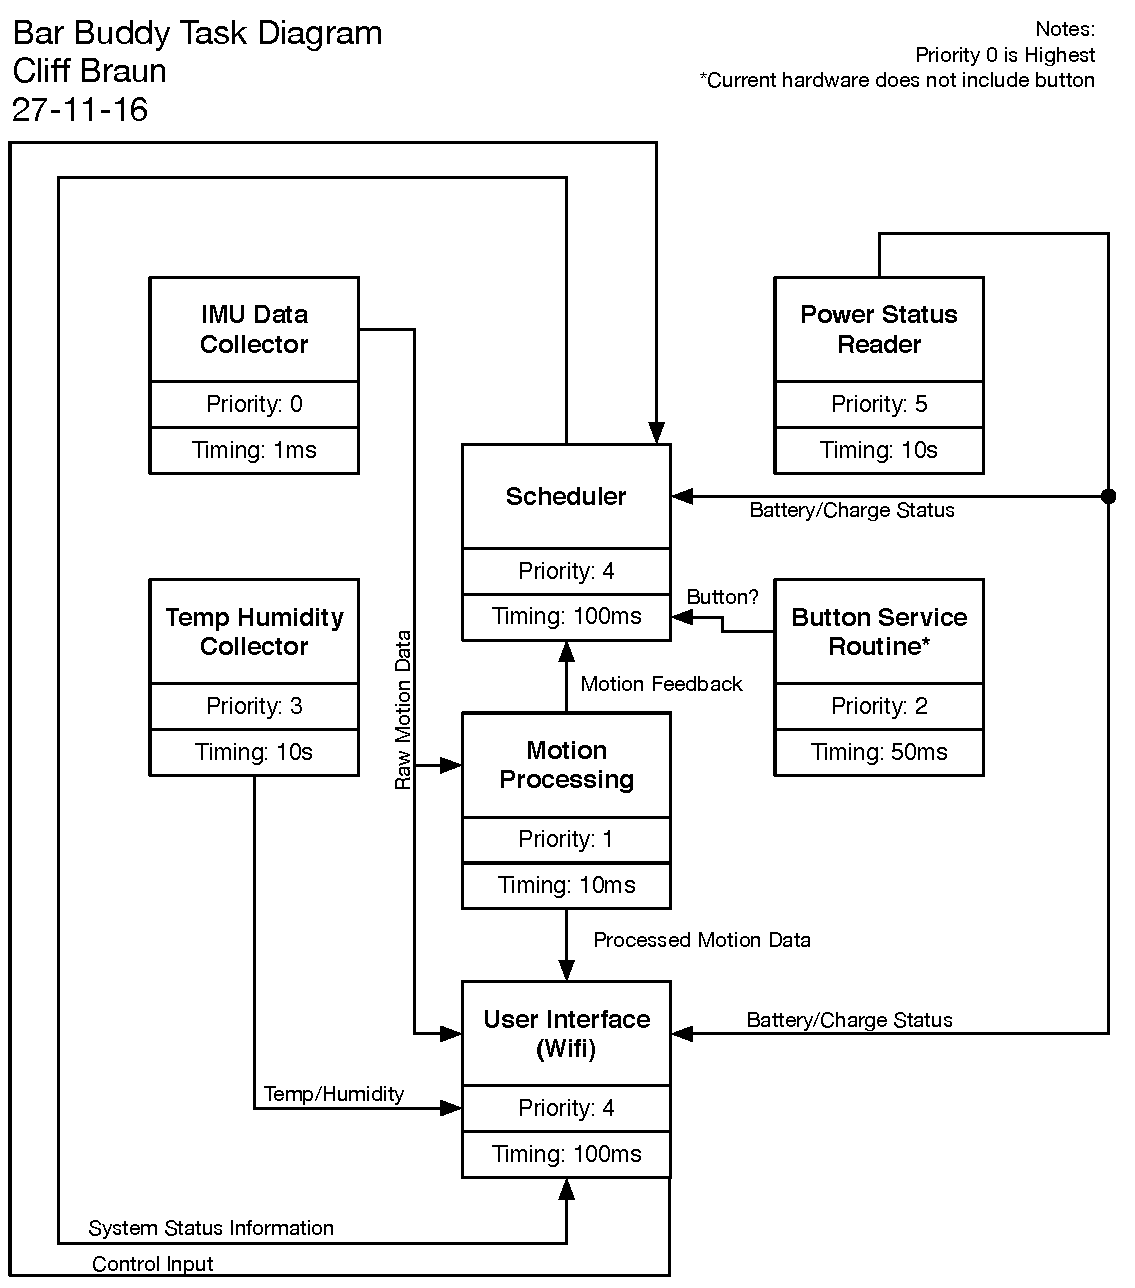
\includepdf[pages=-]{figures/BarBuddy_design.pdf}
\subsection{Proof of Concept Software}
The Beaglebone proof of concept software consists mostly of a rough version of the "IMU Data Collection" routine, along with a utility to plot the resulting CSV files. 

\section{Results}
\subsection{Hardware}
Hardware validation was performed on the major subsystems before the untimely death of the WiPy host. The eagle rendering, and actual board are shown in Figure \ref{fig:board}
\begin{figure}[htbp]
\begin{center}
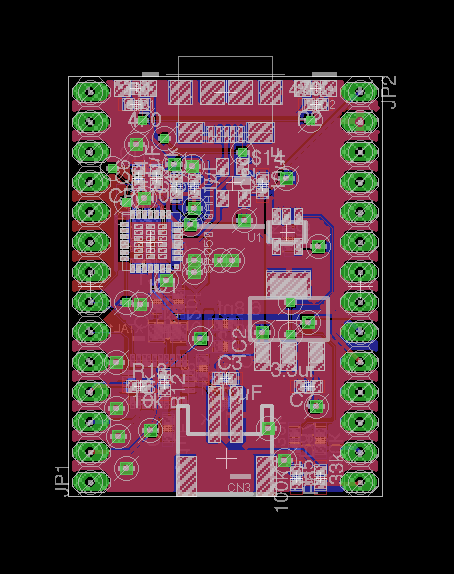
\includegraphics[width=0.4\textwidth]{figures/board.png}
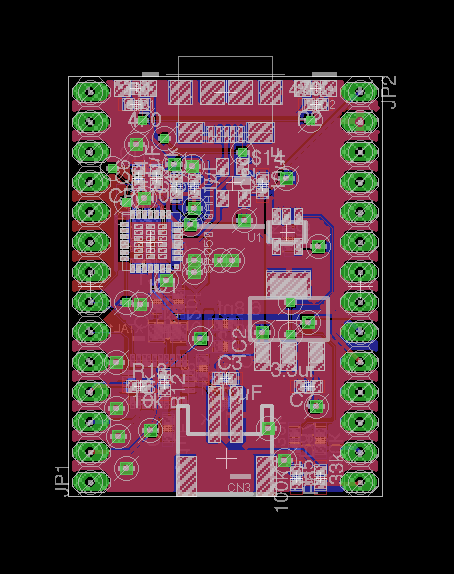
\includegraphics[width=0.4\textwidth]{figures/board.png}
\caption{Top of board: rendered and actual.}
\label{fig:board}
\end{center}
\end{figure}

\subsubsection{Power}
The power subsystem was nearly completely validated. The regulator comes up and provides stable voltages under system loads, but was not tested under loading corner conditions. The LiPo charger successfully charged the system battery, and appropriately actuated the charge signal LEDs. The two analogue inputs of charge state and battery level functioned as intended in the schematic, however an error was discovered in the design: the voltage divider multiplies by 3/4 rather than 1/4. Fortunately the fix for this is as simple as swapping the two resistors.

The major piece of missing validation of the power subsystem is a near-capacity stress test, it is unclear how the device will perform when drawing maximum current, or when attempting to run from a poor power supply. Additionally it is unclear how the system will function when the system is exclusively on USB power without a battery.
\subsubsection{Sensors}
Due to time constraints full validation of the sensors was not performed. 

\subsubsection{Debug}
The CP2102 debug interface was, ironically, the source of most debugging for this effort. The chip is properly connected to the D+ and D- lines of the USB bus, and internal power regulators function properly, however the device will not enumerate on the USB bus of a host computer. Further debug will be performed using a breakout board from Sparkfun as a reference.

\subsection{Data Collection}
Data was collected on one occasion through a bench-press workout in several segments. Overall initial results were very positive, with little processing it is possible to pick out key features. It seems likely that the standard filtering and processing methods applied to activity tracker data will work for the Bar Buddy.

\begin{figure}[htbp]
\begin{center}
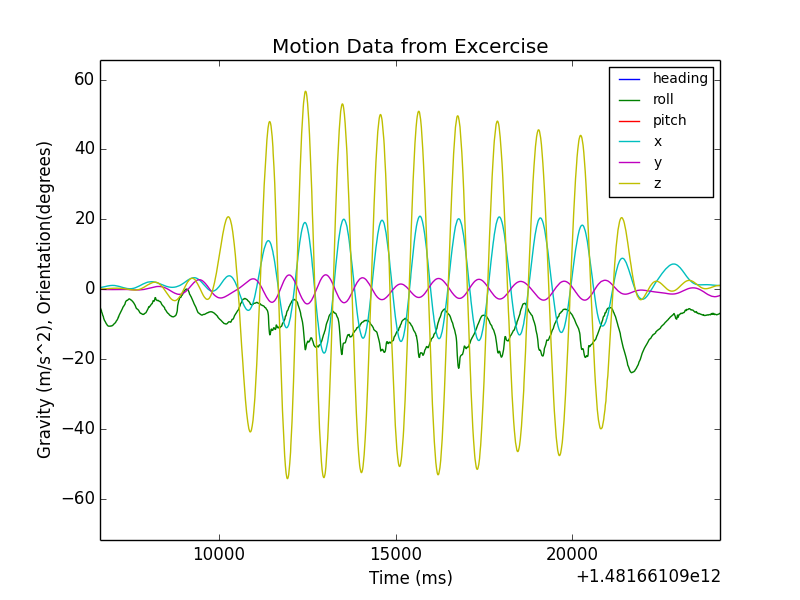
\includegraphics[width=0.7\textwidth]{figures/warmup.png}
\caption{Motion profile of bench press warmup, one set of ten.}
\label{fig:warmup}
\end{center}
\end{figure}

\subsubsection{Warm Up}
The initial recording made with the Beaglebone based Bar Buddy prototype was of a warm-up set of ten repetitions, with only the weight of the barbell (45lbs). Slightly filtered data is shown in Figure \ref{fig:warmup}. The peak-to-peak accelerations in this plot are significantly higher than those in later plots. 


\begin{figure}[htbp]
\begin{center}
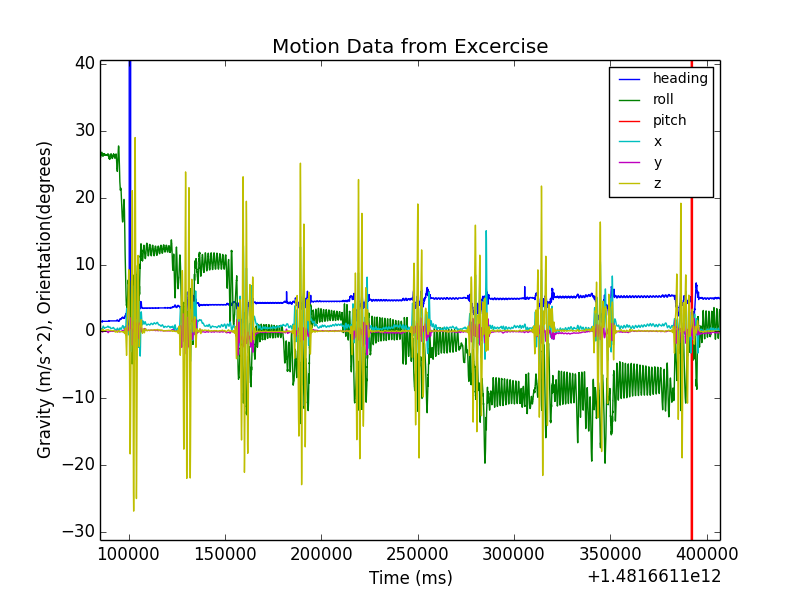
\includegraphics[width=0.7\textwidth]{figures/bench_sets.png}
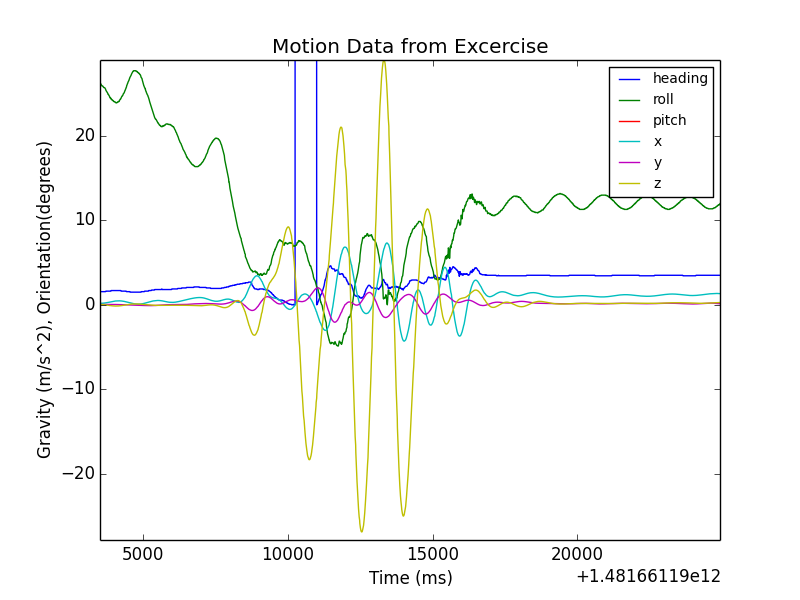
\includegraphics[width=0.7\textwidth]{figures/bench_sets_detail.png}
\caption{Motion profile of ten sets of three bench presses.}
\label{fig:sets}
\end{center}
\end{figure}
\subsubsection{Short Sets}
The next segment of data collected was during ten sets of three repetitions each, performed every 30 seconds. The slightly filtered data is show in Figure \ref{fig:sets}. This plot shows repetitions not quite as cleanly as the previous one, as they were a bit heavier and involved slower acceleration. Two notable features of this plot are the ease of picking out sets of repetitions, and that the acceleration amplitudes decrease slightly as the lifter tires. Figure \ref{fig:sets_heavy} shows a similar set of exercises, but with five sets of two repetitions.  Loading was one again increased, and a corresponding decrease in peak acceleration can be seen. Additionally the last set seems to be cut off somewhat. There was a hard landing, and I believe this may have been a system reset.


\begin{figure}[htbp]
\begin{center}
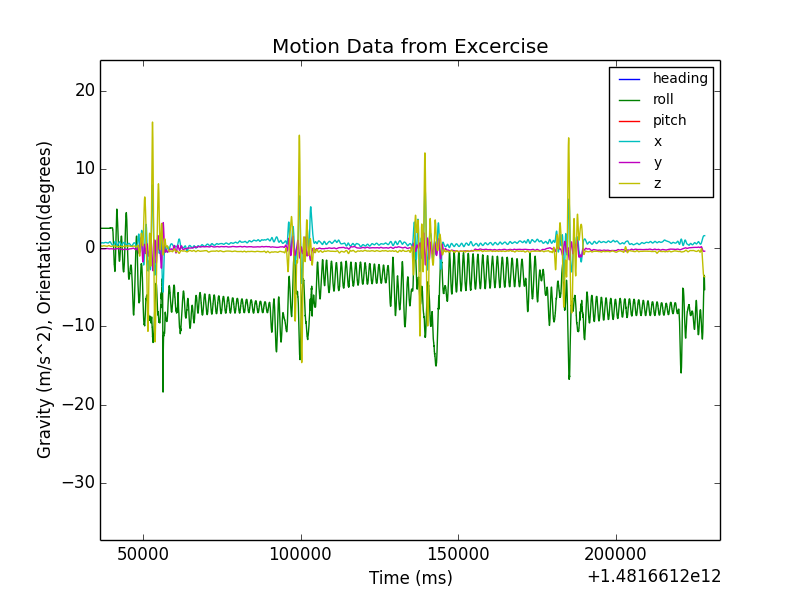
\includegraphics[width=0.7\textwidth]{figures/bench_sets_heavy.png}
\caption{Motion profile of five sets of two bench presses.}
\label{fig:sets_heavy}
\end{center}
\end{figure}

\subsubsection{Paused Squats}
Unloaded squats, with a ~2s pause at the bottom, were performed to examine a slightly different motion profile. The results are shown in Figure \ref{fig:squats}. Because of the pause this data looks a whole lot more messy, and will be more difficult to post-process.
\begin{figure}[htbp]
\begin{center}
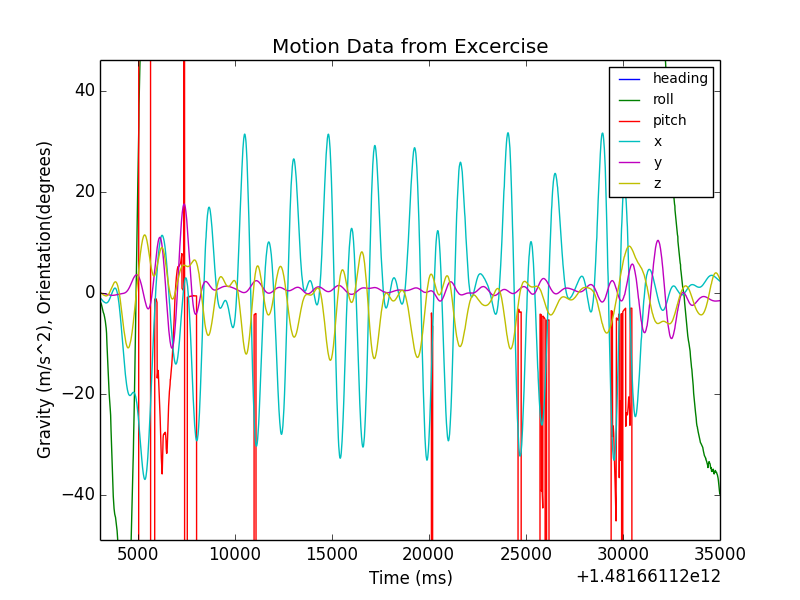
\includegraphics[width=0.7\textwidth]{figures/pause_squats.png}
\caption{Motion profile of paused squats.}
\label{fig:squats}
\end{center}
\end{figure}


\section{Next Steps}
\subsection{Hardware}
\subsubsection{Proto Validation}
Several more validation steps need to be performed to allow for a successful proto-2 release. These are shown in Table \ref{tab:validationtodo}.
\begin{table}[htp]
\caption{Hardware validation todo list.}
\begin{center}
\begin{tabular}{|c|c|}
\hline
Task&Status\\
\hline\hline
I2C Validation& Deprioritized. Hardware allows.\\
\hline
CP2102 & Experiencing unexpected behavior\\
\hline
Si7021 & Deprioritized. Harware allows.\\
\hline
Power Corners & Pending\\
\hline
USB-Only Behavior & Pending\\
\hline
\end{tabular}
\end{center}
\label{tab:validationtodo}
\end{table}%
\subsubsection{Proto 2}
The WiPy appears to have been a poor decision for this product. In addition to being somewhat fragile the documentation and userbase for the device is somewhat less than was expected. Furthermore, a WiPy 2 has been released, so support for the original will continue to get worse.
A new microcontroller will be selected for version 2, ideally one allowing for Bluetooth Low Energy connections to a cell phone to allow use of the device beyond concept validation.

\subsection{Software}
Moving forward the data collection routine will be updated to support whatever platform is chosen for the next hardware revision. The motion processing module will be rewritten to use a Kalman filter to estimate true accelerations and orientations from the noisy sensor output. This data will then be integrated into velocity and position, and finally processed to extract information of interest. 
\newpage
\begin{appendix}
\section{Schematic}
\label{sec:schematic}
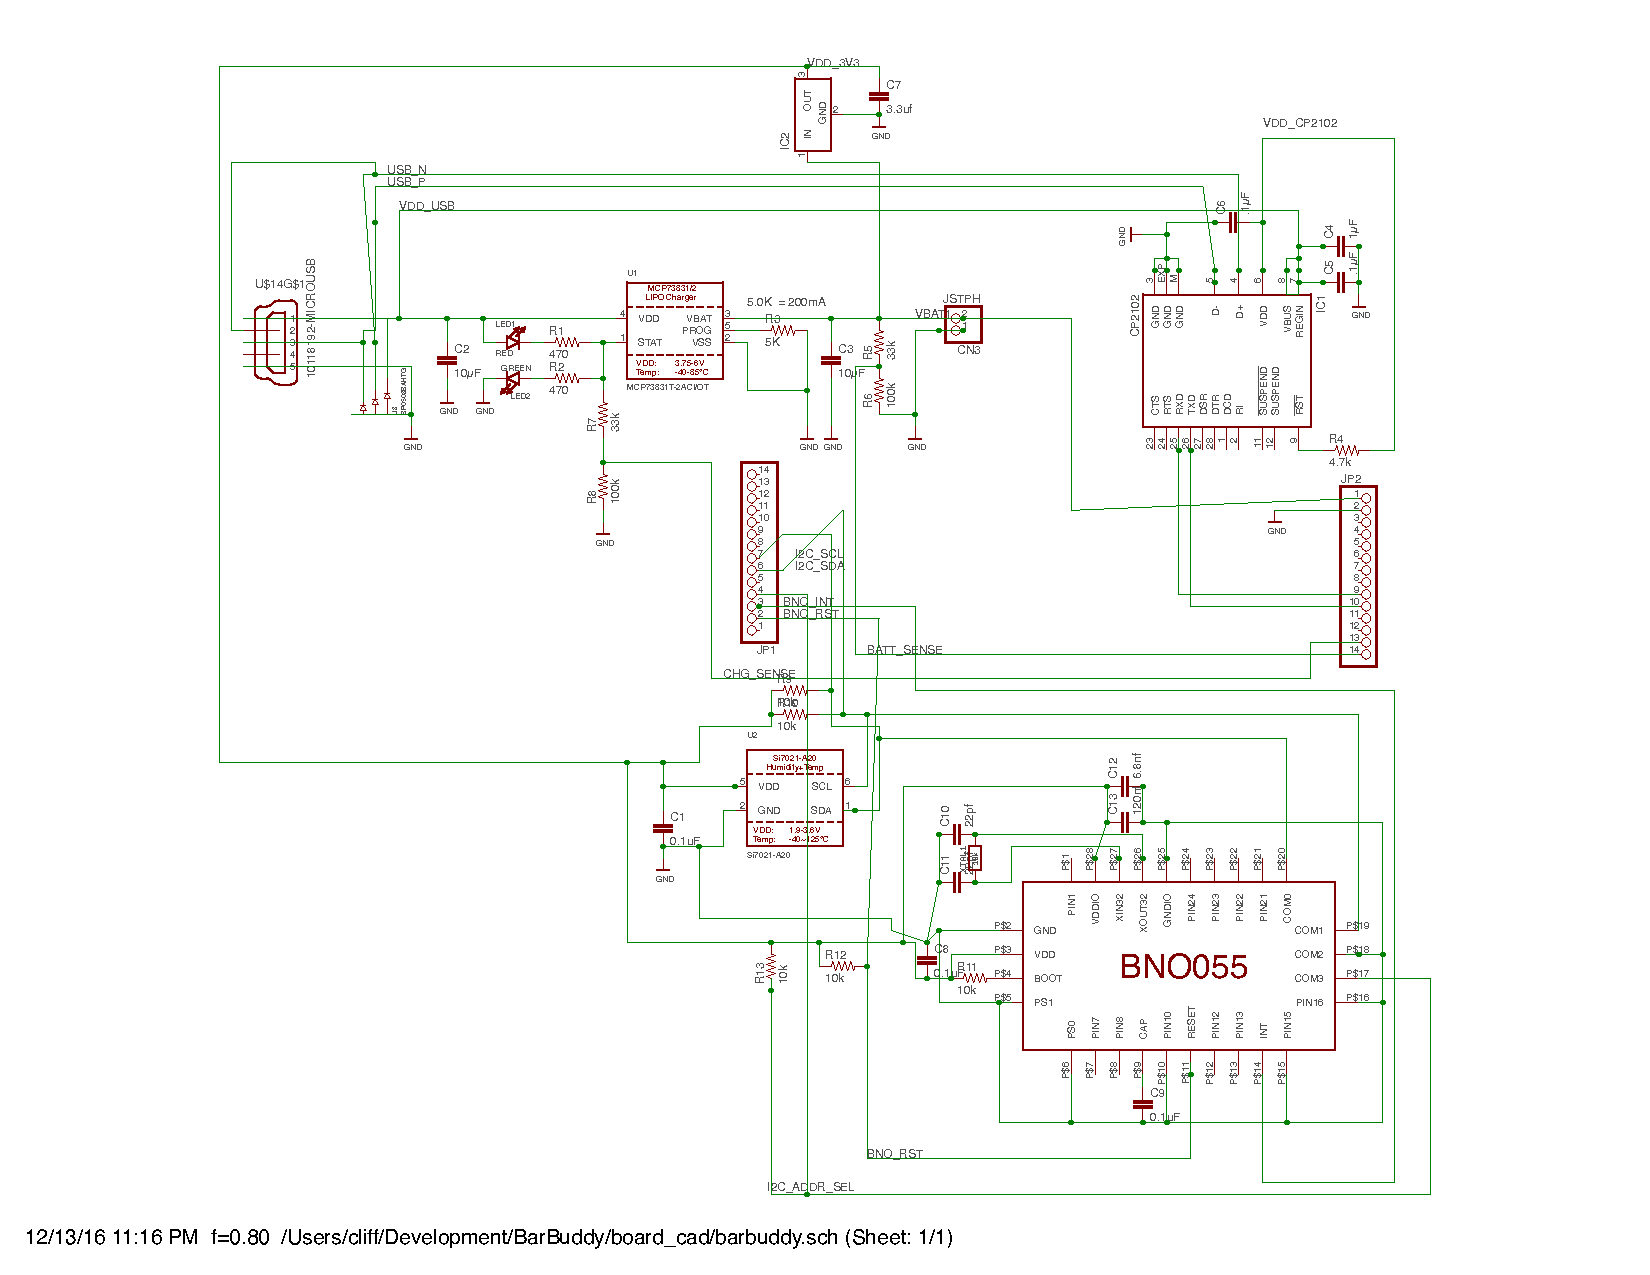
\includepdf{figures/barbuddy.pdf}
\section{Code}
%\subsection{}


\end{appendix}
\end{document}  